\section{Experiment and Analysis}

All below experiments are set up with the Unity engine (version 2022.3.29f1) running on a PC on Windows 11.
The device runs on a CPU of 13th Gen Intel(R) Core(TM) i9-13900HX at 2.20 GHz with 16.0 GB of RAM.

\subsection{Experiment (a): Realism}

To test if the model could realistically simulate the buoyancy force, an experimental simulation immitating the scenario introduced at the beginning of the article where a plank falls into the water is set up.
There are two aspects with which we can judge whether the model is succesful or not:
\begin{enumerate}
	\item Will the plank float back to the water surface and oscillate up and down until it reaches a stable state?
	\item Will the plank turn its flat face up under the influence of the buoyancy force?
	\item If the resistance terms are omitted, will the plank oscillate forever whilst the kinetic energy is conserved?
\end{enumerate}

\paragraph*{Environment Setup}

In an empty scene, a block of static water is placed amid air.
A piece of plank is put above the water surface for a couple of meter's height (figure \ref{simulation-environment}).
The plank's density is made to be lighter than the water density so that it floats.
The water block is wide and deep enough so that the plank would never touch the other faces except the top face.

\begin{figure}[h]
	\centering
	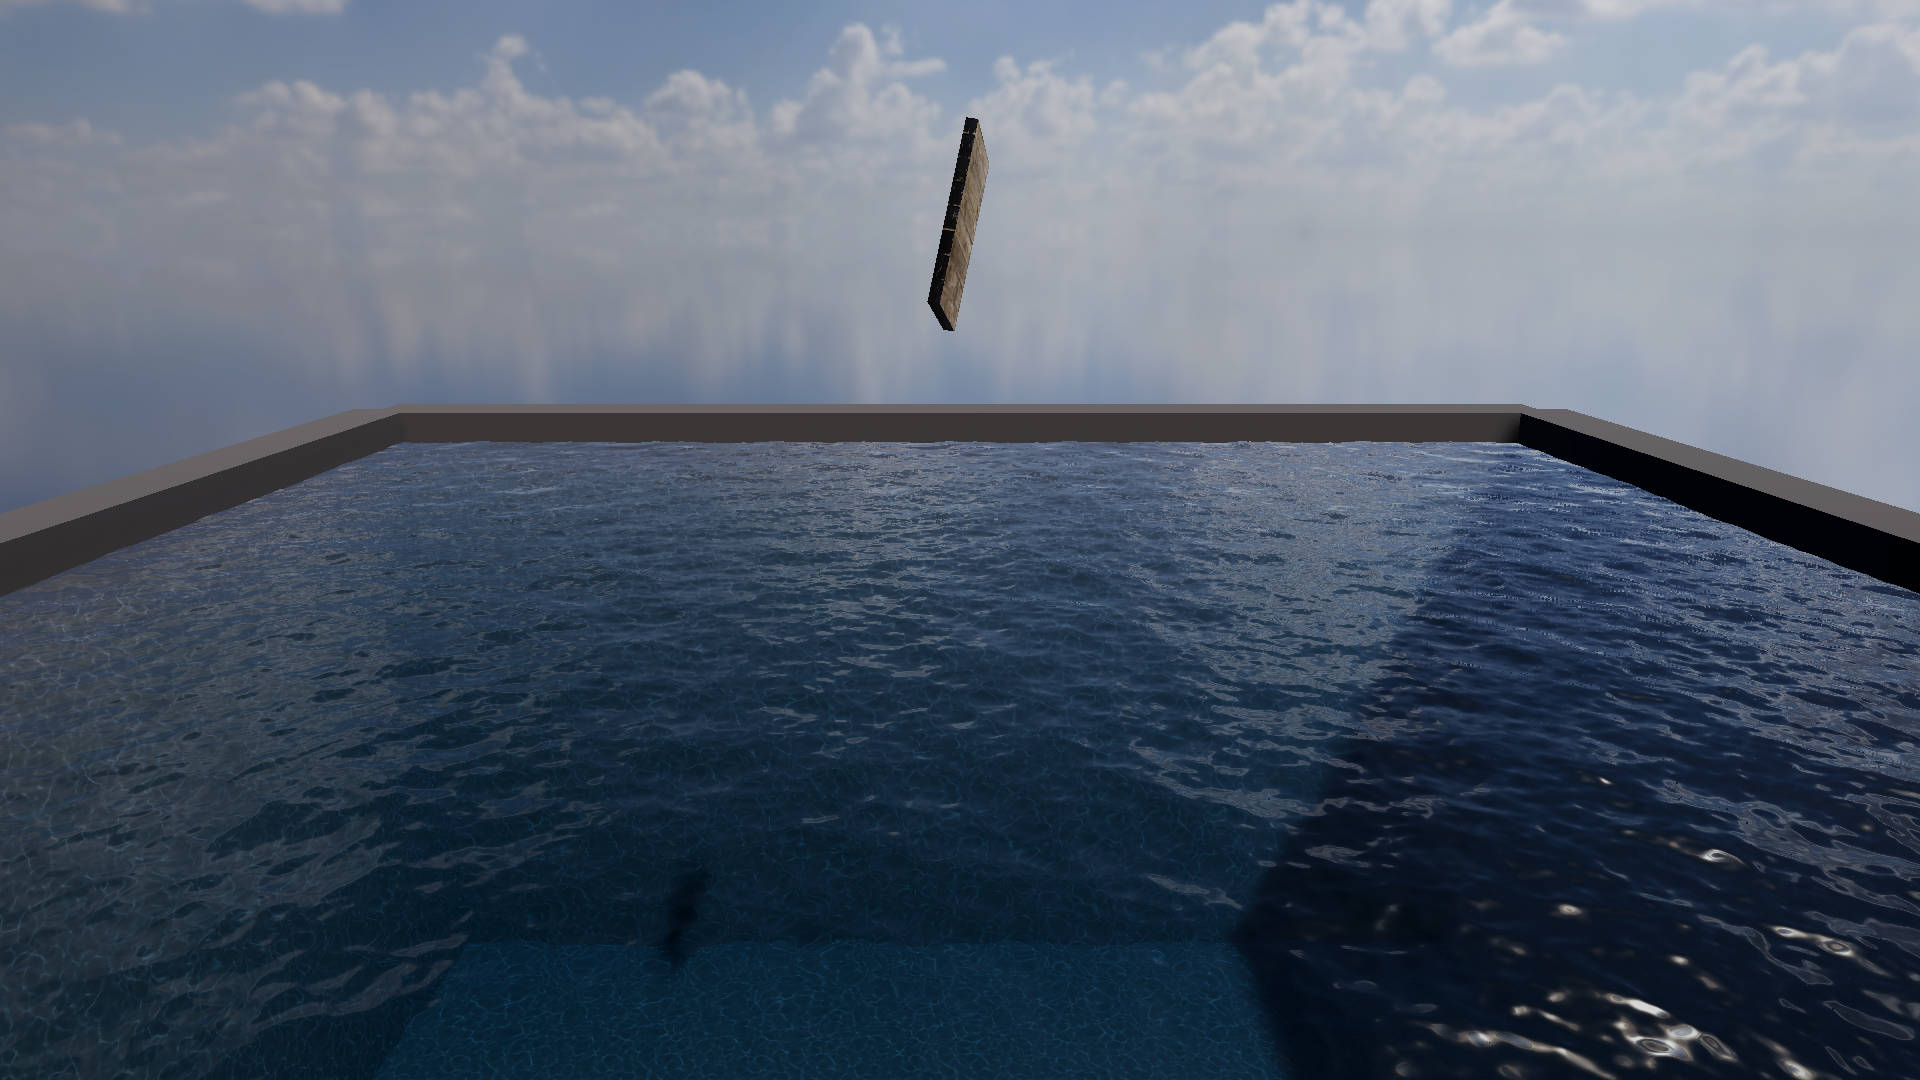
\includegraphics[height=1.5in]{figures/experiment-environment.jpg}
	\caption{The simulation environment.}
	\label{simulation-environment}
\end{figure}

The properties of the water is given in table \ref{simulation-water-properties}.

\begin{table}[h]
	\centering
	\begin{tabular}{ c c c c }
		\hline
		$\rho$ {\footnotesize(density)} & $c_f$ {\footnotesize(form coef.)} & $c_v$ {\footnotesize(visc. coef.)} & {\small dissipation coef.} \\
		\hline
		1.33 & 0.1 & 0.1 & 1.0 \\
		\hline
	\end{tabular}
	\caption{The properties of the water used in the simulation.}
	\label{simulation-water-properties}
\end{table}

The sampling rate is set at 200 samples per surface area per physical frame.

\paragraph*{The Process}

At the beginning of the simulation, the plank is let go free-falling into the water.

During the whole process of the simulation, the critical physical properties of the plank will be recorded in every frame for later analysis.

The simulation will stop at an appropriate time after a relatively stable state is reached.

\paragraph*{Result}

Figure \ref{simulation-result} shows the position and the rotation of the plank relative to the water surface during the fall.
The olive-colored line shows the position of the plank's center-of-mass, the blue line shows the height of the lowest point on the plank, and the red line shows the pitch of the plank's biggest surface -- when pointing to the sky it should be 90$^\circ$.

\begin{figure}[h]
	\centering
	\scalebox{0.65}{
		\begin{tikzpicture}
			\begin{axis}[
				width=5in, height=2in,
				enlargelimits=false,
				xlabel={time (seconds)},
				ylabel={meter},
				ymin=-2, ymax=5, ytick={-2,-1,...,5},
			]
				\addplot[black] coordinates { (0,0) (5,0) };
				\addplot[olive] table[x=t, y=com] {figures/simulation-record.dat};
				\addplot[blue] table[x=t, y=min] {figures/simulation-record.dat};
			\end{axis}
			\begin{axis}[
				width=5in, height=2in,
				enlargelimits=false,
				ylabel={degree},
				ymin=0, ymax=90, ytick={0,15,...,90},
				axis y line*=right,
				ylabel near ticks, yticklabel pos=right,
			]
				\addplot[color=red] table[x=t, y=rx] {figures/simulation-record.dat};
			\end{axis}
			\matrix [draw, below left, fill=white] at (4.25in, 1.25in) {
				\node[olive, font=\footnotesize] {center-of-mass}; \\
				\node[blue, font=\footnotesize] {lowest point}; \\
				\node[red, font=\footnotesize] {pitch}; \\
			};
		\end{tikzpicture}
	}
	\caption{The position and rotation of the plank during the fall.}
	\label{simulation-result}
\end{figure}

From the figures we can see, soon as the plank touches the water surface (the blue line intersects with the black horizontal line), it immediately started to rotate (the red line rises) so that its flat face is splatted onto the water surface;
meanwhile it started perceiving an upward buoyancy force, repulsing it from continuing falling (the olive line starts accelerating upwards).
Eventually, the plank floats up to the water surface and oscillates to a stable state (the olive line tends to be horizontal);
also, the plank's flat face is aligned to the water surface (red line approaches $y=90$).

Figure \ref{experiment-no-resistance} shows a clip of the simulation result when the resistance terms are omitted by setting the drag and  dissipation coefficients to zero.
It can be seen from the olive line that the plank will indeed oscilate forever whilst keeping its kinematic energy.

\begin{figure*}[h]
	\centering
	\begin{tikzpicture}
		\begin{axis}[
			width=6in, height=1.5in,
			enlargelimits=false,
			xlabel={time (seconds)},
			ymin=-5, ymax=5, ytick={-5,0,...,5},
		]
			\addplot[black] coordinates { (0,0) (10,0) };
			\addplot[olive] table[x=t, y=com] {figures/no-resistance.dat};
			\addplot[blue] table[x=t, y=min] {figures/no-resistance.dat};
		\end{axis}
		\matrix [draw, above left, fill=white] at (5.25in, 0.05in) {
			\node[olive, font=\footnotesize] {center-of-mass}; \\
			\node[blue, font=\footnotesize] {lowest point}; \\
		};
	\end{tikzpicture}
	\caption{The resistance-free simulation data captured from experiment (a).}.
	\label{experiment-no-resistance}
\end{figure*}

Based on the analysis of the result, our model has met the desired requirements on realism.

\subsection{Experiment (b): Performance}

The performance of our method could be tested by keep spawning new buoyant objects and tracking the simulation framerate (FPS).

\paragraph*{Environment Setup}

The same water body setup is used, with an automatic spawner dropping planks at a constant rate (Figure \ref{spawner-setup}).
The sampling rate is set to 20 (unit is same as above).

\begin{figure}[h]
	\centering
	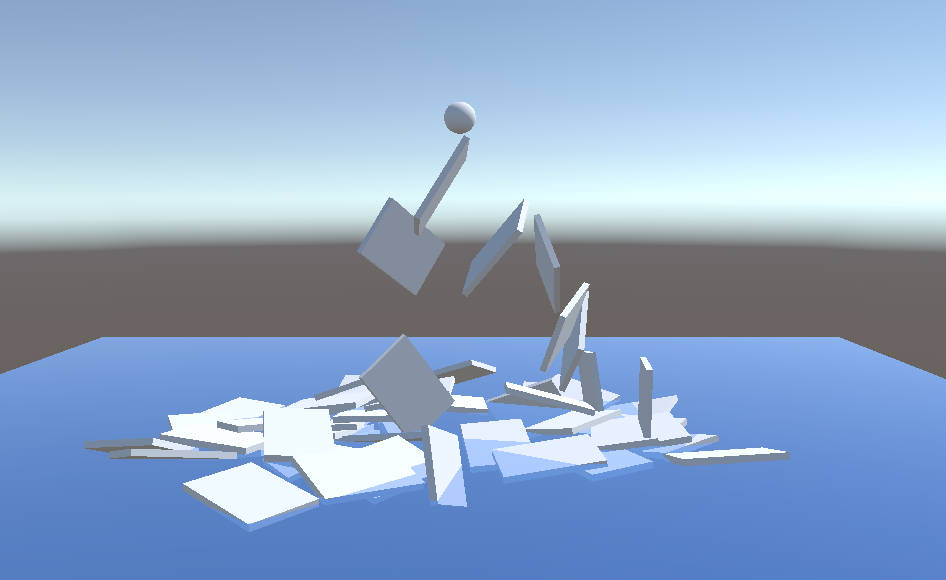
\includegraphics[height=1.5in]{figures/spawner-setup.jpg}
	\caption{A screenshot of the working object spawner.}
	\label{spawner-setup}
\end{figure}

\paragraph*{The Process}

Soon as the scene starts, the object spawner would start working and dropping planks into the water.
The number of spawned planks, the time since start and the FPS corresponding to the time would be recorded in real-time.
Also, we would provide another set of FPS record of the same environment but without the presence of the water body as the comparison in order to clearly see the performance cost caused by our method instead of other environmental factors.

\paragraph*{Result}

Figure \ref{experiment-spawner} shows the change of FPS as more and more planks are spawned and dropped into the water body.

\begin{figure*}[h]
	\centering
	\fbox{
		\scalebox{0.75}{
			\begin{tikzpicture}
				\begin{axis}[
					width=6in, height=2in,
					enlargelimits=false,
					xlabel={time (seconds)},
					xmin=0, xmax=5,
					ymin=0, ymax=500,
					axis y line*=left,
					ylabel=FPS
				]
					\addplot[blue] table[x=t, y=fps] {figures/spawner-real.dat};
					\addplot[gray] table[x=t, y=fps] {figures/spawner-compare.dat};
				\end{axis}
				\begin{axis}[
					width=6in, height=2in,
					enlargelimits=false,
					xmin=0, xmax=5,
					ymin=0, ymax=50,
					ylabel=number of objects
					axis y line*=right,
					ylabel near ticks, yticklabel pos=right,
				]
					\addplot[red] table[x=t, y=n] {figures/spawner-real.dat};
				\end{axis}
				\matrix [draw, above left, fill=white] at (5.25in, 0.05in) {
					\node[blue, font=\footnotesize] {control}; \\
					\node[gray, font=\footnotesize] {comparison}; \\
				};
			\end{tikzpicture}
		}
	}
	\caption{The performance data collected from experiment (b).}.
	\label{experiment-spawner}
\end{figure*}

From the result we can see that our method would cause a linear cost on the performance as the number of submerged objects increases.
At around the time when the amount of objects exceeds 30, it would drag the performance down for about 50\% under the current environment.

In conclusion, our method is suitable for simulations where there are a moderate amount of submerged objects;
it may cause a performance burden if there are too much objects at the same time.

% \subsection{Experiment (c): Complex Geometry}

% The goal of this experiment is to test if our method is working well on target objects with complex geometries, as this is often a disadvantage of other Eulerian approaches that are based on simplified geometries.